\documentclass{article}
\usepackage[T1]{fontenc}
\usepackage[utf8]{inputenc}
\usepackage[brazil]{babel}
\usepackage{graphicx}
\usepackage{hyperref}
\usepackage{fancyhdr}
\usepackage{background}
\usepackage[a4paper,top=3.5cm,left=3cm,right=3cm,bottom=2.5cm]{geometry}
\usepackage{lmodern}
\usepackage{tikz}
\usepackage[font={small,stretch=0.80,it}]{caption}
\usepackage{tcolorbox}

\newtcolorbox{caixa}{colback=red!5!white,colframe=red!60!black}

%Configurando o mapa mental
\usetikzlibrary{mindmap}


%Configurando a path das imagens
\graphicspath{{../../imagens/capitulo3/}}


%Configurando a imagem de background
\backgroundsetup{
scale=1,
angle=0,
opacity=0.4,
contents={
  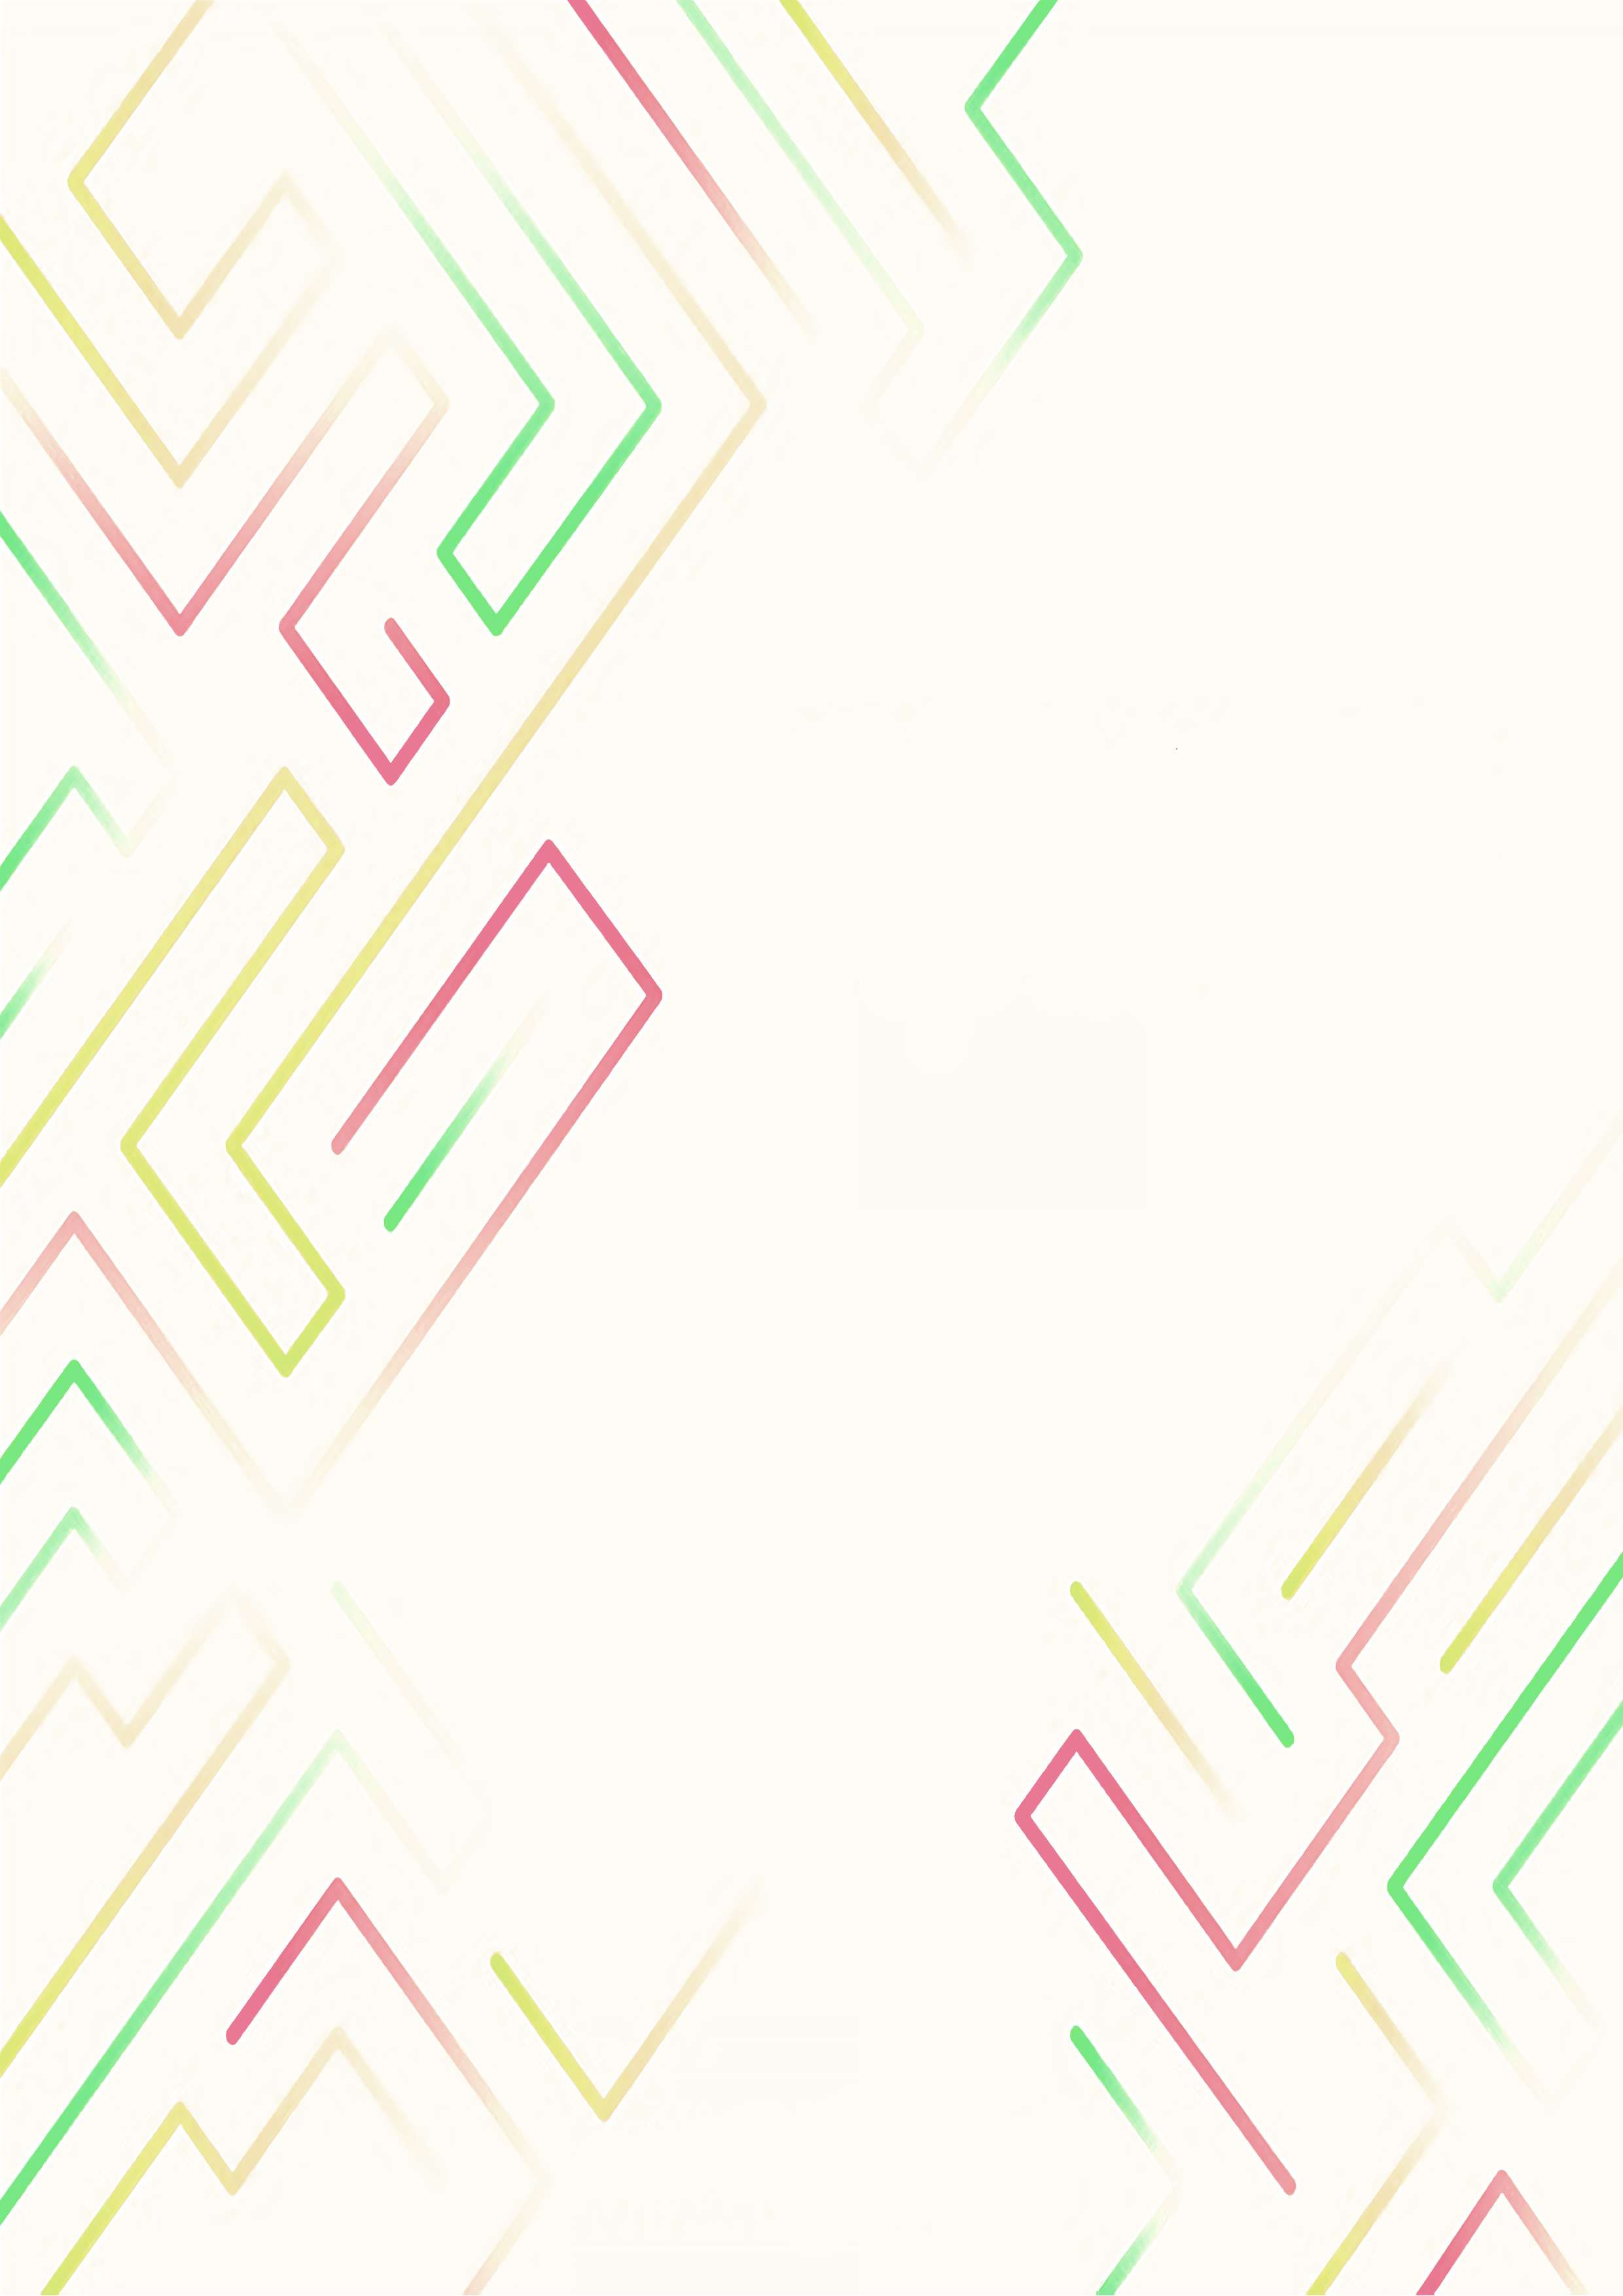
\includegraphics[width=\paperwidth,height=\paperheight]{wallpaper.png}
  }
}

%configurando os hyperlinks
\hypersetup{
    colorlinks=true,
    linkcolor=blue,
    filecolor=magenta,      
    urlcolor=cyan,
}


%configurando os headers
\pagestyle{fancy}
\fancyhf{}
\rhead{LDO}
\lhead{Capítulo 3}
\rfoot{Página \thepage}

%configurando identação e separação de parágrafos
\parindent 1.27cm
\parskip   6pt

\flushbottom

%títulos,autor e data
\title{\textbf{Capítulo 3 \\ Como é feito o aprendizado de máquina}}
\author{Homenique Vieira Martins}
\date{Novembro de 2020}



\begin{document}
    
    %Inserindo o título
    \maketitle

    %Mapa mental
    \begin{center}
      \begin{tikzpicture}[mindmap, grow cyclic, every node/.style=concept, concept color=orange!40,
        level 1/.append style={level distance=5cm,sibling angle=105},
        level 2/.append style={level distance=3cm,sibling angle=55}]

        \node{Aprendizagem de maquina}
        child [concept color=yellow!30] { node {YouTube \\ \ref{sec:youtube}}
        child { node {\href{https://www.youtube.com/watch?v=Lu56xVlZ40M}{IA quebrado o jogo}}}
        child { node {\href{https://www.youtube.com/watch?v=sw7UAZNgGg8&t}{O jogo que fica mais esperto}}}
        child { node {\href{https://www.youtube.com/watch?v=QOJfyp0KMmM}{Machine Learning destruindo no Tetris}}}
              }
        child [concept color=teal!40] { node {Feramentas \\ \ref{sec:feramentas}}
        child { node {\href{https://cloud.google.com/vision/}{Google Vision AI}}}
        child { node {\href{https://www.tensorflow.org/?hl=pt-br}{tensorflow}}}
              }
          child [concept color=purple!50] { node {Leituras \\ \ref{sec:leituras}}
        child { node {\href{https://www.datageeks.com.br/machine-learning/}{Machine Learning para todos}}}
        child { node {\href{https://bityli.com/hGR18}{Supervisio nada ou Não?}}}
              };
      \end{tikzpicture}

    \end{center}

    %Configurando pagina
    \newpage   

    \begin{caixa}

      \begin{center}

          \href{https://soundcloud.com/gustavo-rodrigues-468052117/ldo-machine-learning-capitulo03}{Ouça o Podcast desse PDF!}

      \end{center}

    \end{caixa}

     %Iniciando a seção 'O que é'
    \section{O que é?}
    \paragraph{}
    Pode parecer estranho a ideia de ensinar uma máquina a aprender algo , porém o machine learning nada mais é 
    que uma maneira diferente de tratarmos os problemas computacionais. Onde antes o programador tinha que pensar 
    em todas as soluções possíveis para um determinado problema agora a própria máquina pode gerar boa parte ou quase 
    toda a solução para um problema. isso tudo é possível graças a certas técnicas de aprendizado de máquinas, neste 
    LDO eu vou apresentar para você as 3 técnicas mais populares nos dias de hoje.    

    % 01 - Aprendizado Supervisionado 
    \section{Aprendizado Supervisionado:}
    \begin{figure}[ht]
        \centering
        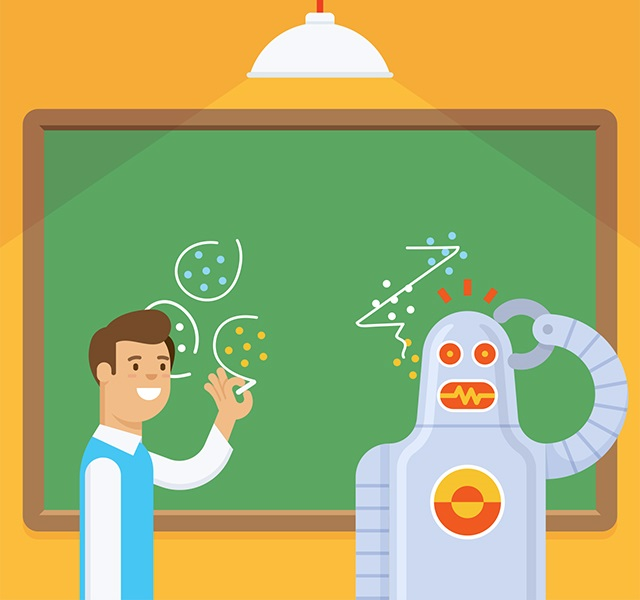
\includegraphics[scale=0.3]{robo_aprendedo.jpg}
    \end{figure}
    \paragraph{}Vamos dizer que você quer que uma maquina aprenda a reconhecer o que é um gato, para isso você
    precisa mostrar para ela varias fotos de gatos e coisa que não são gatos e informando-a a mesma aquilo que é um gato 
    e o que não é um gato, depois de uma certo numero de rodadas a maquina vai começar a reconhecer padrões que vão indicar que 
    algo pode ser um gato com mais ou menos uma certeza, porém ainda sim podendo errar, 
    esse estilo de abordagem é conhecida como aprendizado supervisionado. Onde você informar para máquina os dados( informação,
     foto e etc) e junto a ao dados você também rotula os mesmos para a máquina entender qual é o objeto que ela está sendo
     estudado.  
    Essa abordagem é excelente para situações onde existem um padrão conhecido e você quer a máquina 
    reconheça e possa atuar em cima disso.

    \newpage

   % 02 - Aprendizado não Supervisionado 
    \section{Aprendizado não Supervisionado:}
    \paragraph{} Agora você não quer rotular nada, mas quer a máquina diferencie por si só o que ela encontra
    e separe em grupos que ela acha que seja parecido, isso é um aprendizado não supervisionado.
    Onde a máquina só tem os dados, porém ela tem que classificar cada objeto a partir de um
    conjunto de variáveis  que ela acha que sejam parecidas. 
    \\
      \begin{figure}[ht]
        \centering
        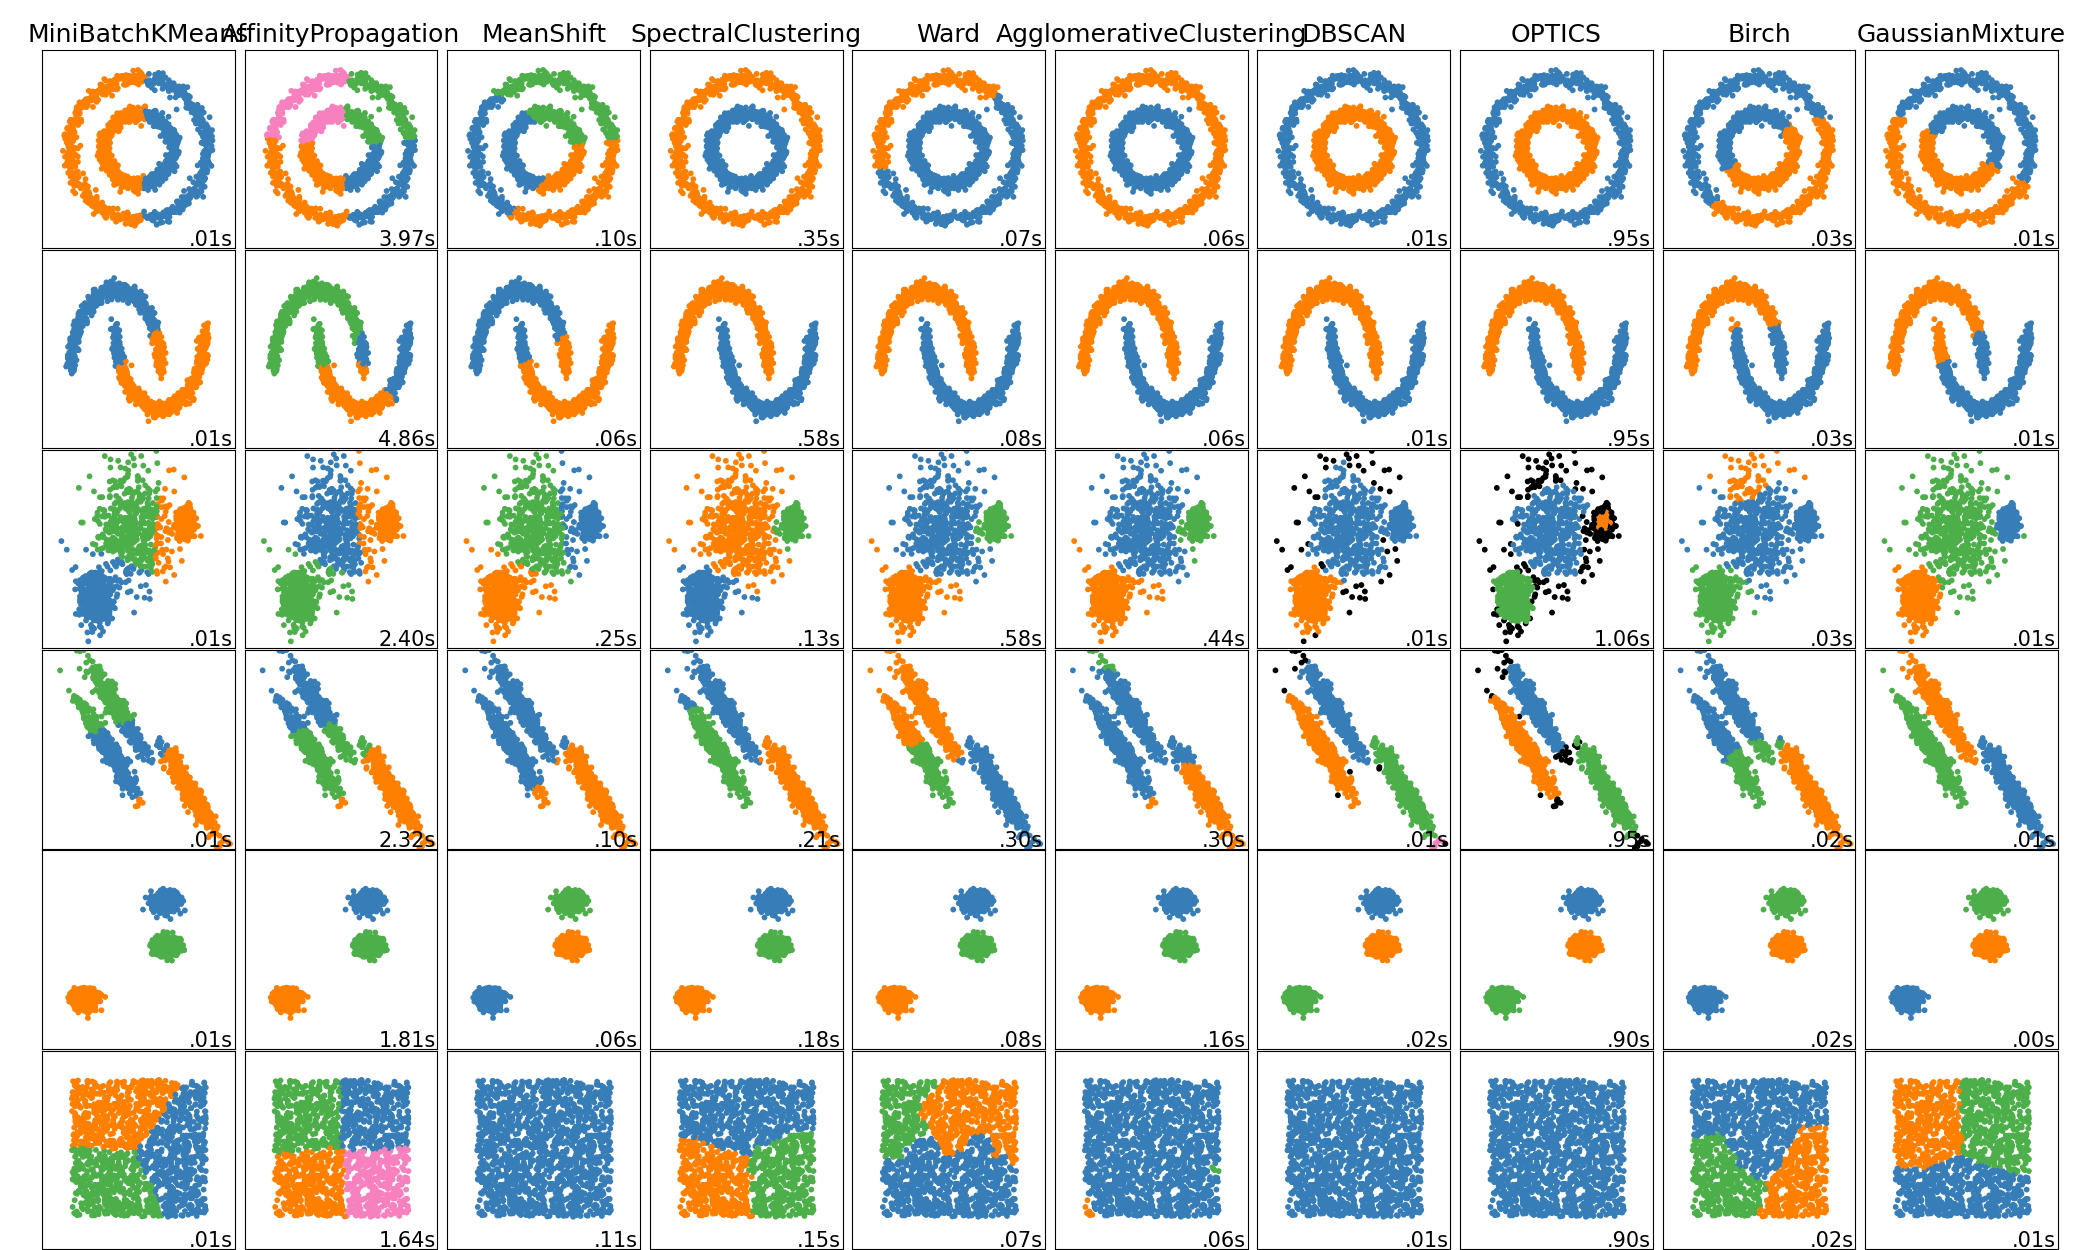
\includegraphics[scale = 0.25]{classificação de grupos.png}
    \end{figure}
    \\
    Pegamos por exemplo a Amazon,
    ela tem vários clientes com gostos diferentes, porém ela quer saber qual produto recomendar para um determinado
    cliente que almente a chances dela vender o produto ou qual é a melhor tipo de abordagem para determinado 
    tipos de clientes. Esse tipo de análise,pode ser muito bem feito por esse tipo de abordagem de aprendizado   

    % 03 - Aprendizagem por reforço
    \section{Aprendizado Por reforço:}
    \begin{figure}[ht]
        \centering
        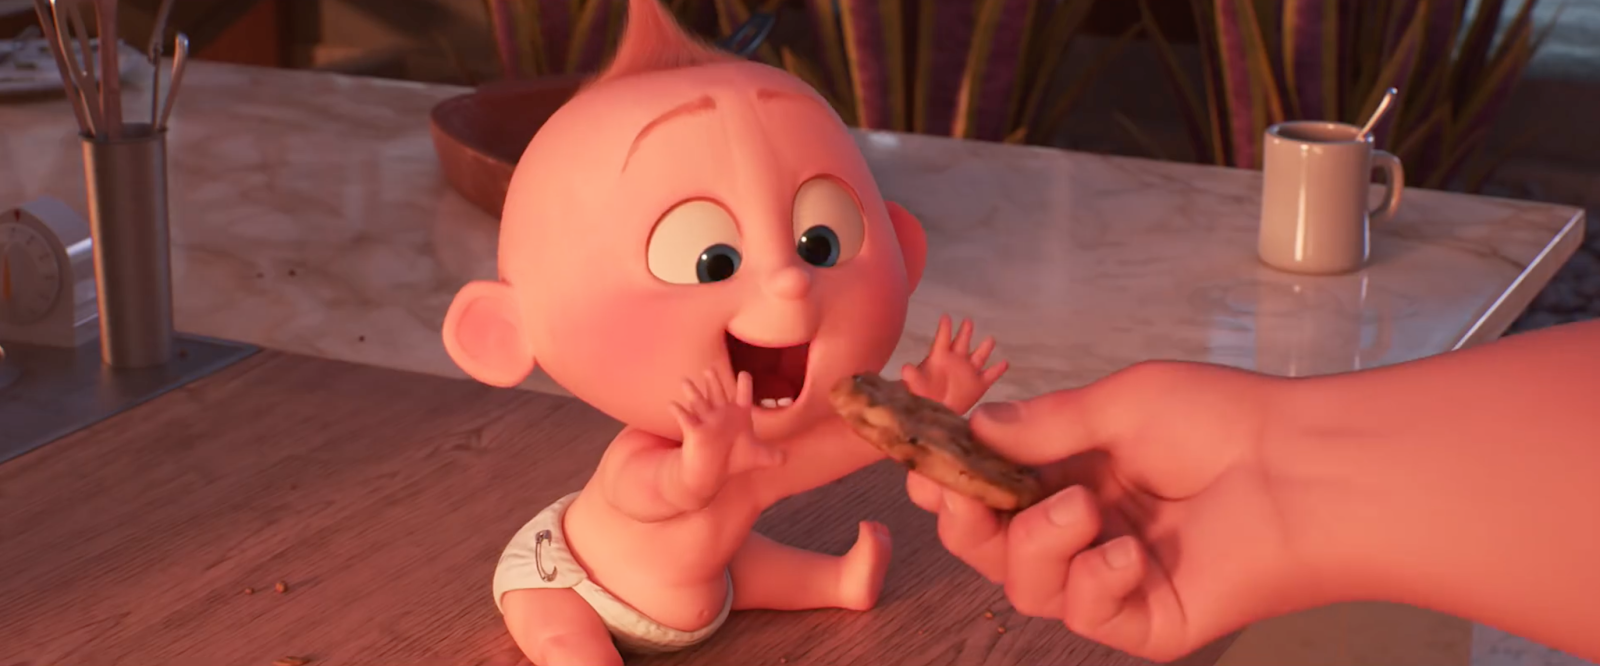
\includegraphics[scale = 0.2]{jack-jack-num-num-cookie_orig.png}
    \end{figure}

    \paragraph{}Aprendizagem por reforço é uma área de aprendizagem de máquina que investiga como a maquina devem agir em determinados 
            ambientes de modo a maximizar alguma noção de recompensa cumulativa.

    \newpage 

    % 04 - Sessão Extra  
    \section*{\centering Extra}
    Quer ver mais um pouco sobre o Machine Learning?
    \begin{itemize}
        \item\href{https://www.youtube.com/watch?v=R9OHn5ZF4Uo&t}{How Machine Learn(Com legendas em pt-br)}
        \item\href{https://www.youtube.com/watch?v=mhe5e2B9bL8&t}{Machine Learning: como ensinar uma máquina a aprender | Nerdologia Tech}
        \item\href{https://www.youtube.com/watch?v=r8KWciNmEGw}{(Aprendizado por reforço)Inteligência Artificial ESTACIONANDO carros!} 
        \item\href{https://blog.wittel.com/o-que-e-machine-learning/}{O que é machine learning e quais são as suas aplicações no mercado?}
    \end{itemize}

    \clearpage
    %Bibliografia
    \begin{thebibliography}{2}
    
    \bibitem{Nerdologia}
    Atila Lamarino \\
    \href{https://www.youtube.com/watch?v=mhe5e2B9bL8&t}{Machine Learning: como ensinar uma máquina a aprender | Nerdologia Tech}

    \bibitem{CGP}
    CGP Grey \\
    \href{https://www.youtube.com/watch?v=R9OHn5ZF4Uo&t}{How Machine Learn(Com legendas em pt-br)}

    \end{thebibliography}    
\end{document}